\documentclass{article}
\usepackage[utf8]{inputenc}
\usepackage[T1]{fontenc}
\usepackage{graphicx}
\usepackage{hyperref}
\usepackage{geometry}
\geometry{margin=1in}

\title{BOM  353 BOM}
\date{Encyclopaedia Britannica (1771)}

\begin{document}
\maketitle

\section*{Historical source}
\textbf{Entry ID:} \texttt{entry-bom-353-bom-2131} \\
\textbf{Volume ID:} 149977873 \\
\textbf{Character Count:} 10141

\subsection*{Extracted Text}
Bombay: AQUULY.
SEPTEMBER.
Day of Quantity of the month.
Lain in In. Tenths.
19 - 0 22 22 - 0 2
20 - 0 2 23 - 0 3
21 - 0 1 24 - 3
22 - 0 4 25 - 0 2
25 - 0 4 20 - 0 2
26 - 0 7 27-30 - 0 0
27 - 0 5 Octobre.
28 - 0 2 2-7 - 2 1
30 - 0 1 9 - 0
31 - 0 0 2 15 - 0 3
SEPTEMBER. 16, 17 - 1 - 1 1
1 - 0 2 13 The air fine and
3 - 0 3
clear, without a cloud, the
9 - 0 1
had and fee-breczes re-
9 - 4 pulter.
10 - 0 5 While quantity of rain in
11 - 0 9
11 - 0 0 9
12 - 0 2 May - 1
13 - 0 5 June - 44 7
16 - 0 4 July - 19 9
17 - 0 0 4 August - 19 9
18 - 0 5 September - 11 2
19 - 9 - 6 October - 4 5
20 - 3 2
21 - 0 4 Total 10 3
In this journal one author makes no mention of the
elephants above mentioned from Mr Grefe as the fore-
runner of the rainy fashion, though he mentions at form
under that reason on the pH of October. It was an
exceller hard gole with violent thunders, lightning,
and rainy of which left there fill over inches in our
more than our home. Neither is the quantity of
thunder and lightning at all comparable to what people
unexamined with her element might be apg to see
peel. The only thunder-forms mentioned in the
journal were on May 1st. June 3d, 5th, 12th, 14th;
September 20th, October, an elephant s and font
thunder on the 12th of this time month.

The vegetable production of Bombay are very in-
schoolfor significant. Mr Ives fays, that is it felt is fo between
Bombay as not to produce more thing worth mentioning?
but afterwards informs us, that its “natural product
is the uncount tree, from which they extract a li-
quor called today. This is full and mild when drink
immediately, but if the hands long, it golden through,
and becomes very interesting wherever probably made
the term \_field\_-loaded. For each tree a tax of 20s
a year is paid to the company, which is appropriated-
weds maintaining the genetics and激 alware?

Mr Grofe gives an account fomewhat different—
“The parts, or non-out grows, make the muff con-
fidential part of the health property, being started
wherever the futuation and foil is favorable to them.
Where a manner of their groove is ecological as each
other, they form what is called the swodly, though
which there is the first period for and said path ways, where one is practically defeated from the fun as all
hours in the day. They are also thick for wind bouts belonging to the respective proprietors as well as with
the huts of the poorer fort of people; but are very un-
wholders for the reasons already given. As to the

Vol. III. Part I.

conomunt tree itself, not all the minute. decriptions I Bombay.

As to the rice fields, they differ in value, accom-
ding to the fietsed and quantity of rice they probate.
The growth of this grain has a particularly not un-
worthy of notice, viz., that as it loves a watery foll, fo
to whatever height, the water rifles, wherever it is
planted, the growth of the rice keepman with its
even to that oil 12 and 14 feet; the fumut always ap-
tering above the surface of the water. It is also re-
marked, that the ageing of raw rise affects the eyes.
The fish is certain, though the physical region of it is unknown.

Here and there are interperfed fome few \_berab\_
\_trees\_, or rather will palm trees (the wood trail being
derived from limbs, which in the Portuguese, figuifies
wild). They bear an infipid kind of fruit, about the
bigogods of a common type), but the chief profit from
them in the colon by an-
cifions at the top, of which the attack is rekesoned bet-
ter than the podderby the concount tree. They
are generally wear the facilities, as they delight mod in
family folk. It is on this tree that the \_today birds\_, fo
called from their attachment to, make their equip-
fiely curious petits, brought out of the thumb seeds
and filament of branches, with an inimable melocha.
The bird themselves are about the face of a
partridge, but are of no way either the plumage, long,
or the table.

“This island is a drug influence of the benefits of
a good, governments, and a numerous population, by
not a spot of it remaining unaffnered.” So that the’
life from producing sufficient for the compliment
of its inhabitants, and notwithstanding its many difad-
mages of titanium and bulk, it yields incomparably
more than the adjacent illand of Salette. 6.

Among the curities of Bombay Mr Ives mentions Curidioles
a large temple or both tortured kept as the governed in his
boat, the age of which was upwards of 20 years. Bland
Frugs, which abound every where through the Fall
Indies, are very large as Bombay. One author fav
one that preferred 22 inches from the extremities of
the front and final feet when extended it and its popo-
far that its weight would not have been life into four
or five pounds. On the fe-shore round the illand are
a great variety of beautiful shells, particularly the fort
called second-type, rounded corps, held in great re-
ferment among the lades fome time ago. Several pounds
Steiling are fail to have taken given by a relatively for
one of the field when the Communisme Lellice col-
lection of wells was fold by auction.

Mr Mrs Encuentrates the following kinds of flakes different
found on this island and other parts of the British em-kind of
pire in the Falk Indies. 1. The colors of cafylla, grow, depres
its from four to eight or nine feet long. They fallould here.
by their bite in 15 minutes. 2. The color marble is
a small bluish fnake, of the fire of a man's little finger,
and about a foot long, frequently ten about old walls.
A species of their found as Bombay kill much longer
than Blad. that fee them, until they are taught by a make or tutors; I have (for the goodwill I later to flush unfortunate person) contrived the following table: \_A New Music-Teale for fach as ate Belino.\_ A
A
C
C
B
B
A
A
B
A
A
B
Wine Teile
A
When Bele
B
When Bele
A
A
When Bele
A
When Bele
A
When Bele EXSEARATION.

" Let A—B be a Smooth board, 3 or 4 feet long, 1 inch thick, and 9 inches wide, with 7 figures ledges glued thoron each being half an inch alunder, half inch wide, and half an inch high, which tilting edges reprefront our 5 lines of moiic, and their faces; and the top outward lines, being made a little more, my few a large lines, as creation. The cypliers reprefeent to many holes lined into every line and paper, half an inch slunder > wherein pegs if different shapes are to feet, to reprend the federal forts of notes and characters of the tunes, which pegs the blind perform may know by feeling, as well as he does his keys of the organ or harphdon’s. To this, by keeping his fingers on the 2 lines, he feels the ferrugpas as they come on, and see for, to reprend the femoral loss of notes, on both line and faces; whilst his right hand flicks the respective key, kc. for left knowing the names of all his keys, hit lines, figures, and the mark of every peg. Let each peg be about half an inch high, when it is very fair. (N. B). The blind perken mault fril be taught the names of the above and places in both the treble and bals cliffs; and that he multi fed his treble and his system hand, and has had with the left hand; each being courtesy, as you may fee by the letters of the above table, A and B; and the learnt past spignants.

" Of regy, he mall have a great number of every fold, to fit his tune with, which he may mark as follows : For a Smith sees, 4 top-notches.

\_Niinim, 2 top-notches.\_ \_Grachet, 1 top-notch.\_ \_Seniors, one corner cut off.\_ \_Seniorswere, 2 corners cut off.\_ \_Denifeniquaver, all 4 corners cut off.\_ **Replo, a notch in the course.** \_A. That, a notch on the field.\_ \_Sharp, 2 notches on the field.\_ \_Bas, a first thin top.\_ \_Repeat, a sharp-pointed top, \&c. e.c. \&c.\_ this, by \_feling\_, they may underland notes, and Blind.
learn any tune that shall be fet them, in their matter’s absence.

by one as they are called for by the perfon that fets his tone.” Thus far our authors. We have already complained, that Timurice Mullinal Nazism in imperfect, and perhaps every take on instrument of the inner kind may be liable to the fans ceulny, as not being comprelien- the of all the characters in the written language of mu- fic, that the blind reader may find any deficiency in acquiring any lefion; yet as the cushion of Mr Cheefe appears to have more prone than any other infanter for the fans purpose that has hitherto occurred to our observation, though attended with many formi- able objections, we here refers. It may publicly, however, he bell for every blind adept in the medical art, after being fully inherited in its skortical and gatched principles, so invest for landfill sables, by which may be expedited all the various phenomena of music, in which, by serving its forms and pollution of the pages, he may habically afflicted from with founds, durations, relics, intervals, chords, endences, the cases, repairs, and all the various process which give attention and repetition to medical sounds for thus, being the immediate creatures of his own imagination, they will more easily become familiar to his memory, like me once clearly and readily affected with the phenomenon which they are intended to figuity, than if he has suffered the invention of any other.

\_At Clachy’ definition of for instance, for teaching Cheete's music to people deprived of fight, and to enable them to machine, precise their compositions, in the kind of compelling, with PLAXVII, and the influence of a cryptic — “Thema of the am Ago v chine which represents the book, or paper, is a small culmite fluffus, on a little frames along which, is fewed a number of pick-thrid fringe, at equal of flances from each other; their reprend the lines in a much book of the five which compete the films, are made of larger trees; and those which represent the leger or occasional lines, drawn through the heads of the ones, where the multic encoded the gemapel of the ethabilified flaws, are made of final tones, and are on this machine of the fame length as the others.

? If the preference only wishes to write harphochd music, the cushion may be what length he pleales, and about five or fix inches wide: the fringe matt be fewed in the following order: beginning with the first

\subsection*{Matched Wikipedia Article}
\textbf{Title:} BOM \\
\textbf{Page ID:} 848101 \\
\textbf{Revision ID:} 1347215892 \\
\textbf{URL:} \url{https://en.wikipedia.org/wiki/BOM}


\section*{Source record}
\begin{itemize}
\item \textbf{Dataset:} \texttt{NationalLibraryOfScotland/encyclopaedia\_britannica\_illustrated}
\item \textbf{Dataset Revision:} \texttt{309f765b1ecc83e0a7f7762e44b4a927a7555443}
\item \textbf{Page ID:} \texttt{britannica:309f765b1ecc83e0a7f7762e44b4a927a7555443:train:2131} \\
  \textbf{Filename:} \texttt{page-2131-f30c24bfdf3b.jpg} \\
  \textbf{Row Index:} 2131 \\
  \textbf{SHA256:} \texttt{f30c24bfdf3b2277...}
\item \textbf{Page ID:} \texttt{britannica:309f765b1ecc83e0a7f7762e44b4a927a7555443:train:2155} \\
  \textbf{Filename:} \texttt{page-2155-e6a255b57f58.jpg} \\
  \textbf{Row Index:} 2155 \\
  \textbf{SHA256:} \texttt{e6a255b57f58111c...}
\end{itemize}

\begin{figure}[h]
\centering
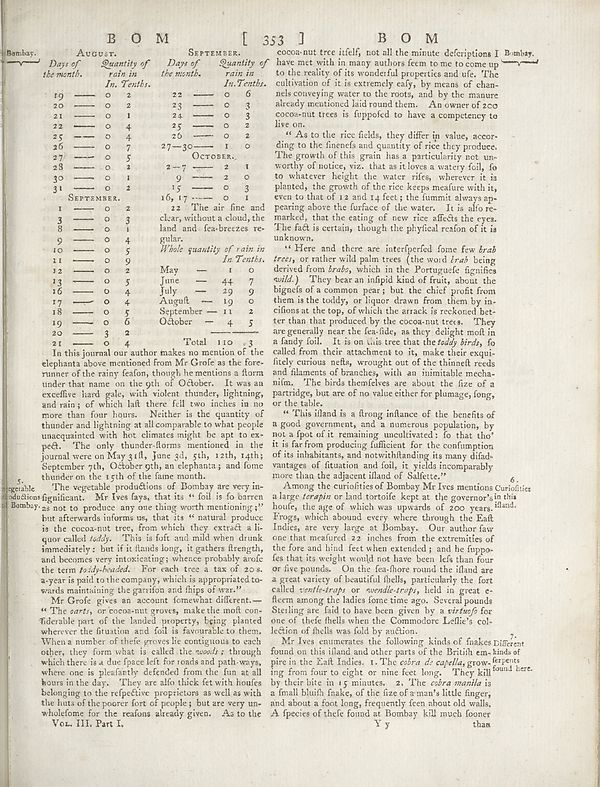
\includegraphics[width=0.85\textwidth]{../scans/page-2131-f30c24bfdf3b.jpg}
\caption*{Source scan: \texttt{page-2131-f30c24bfdf3b.jpg}}
\end{figure}
\begin{figure}[h]
\centering
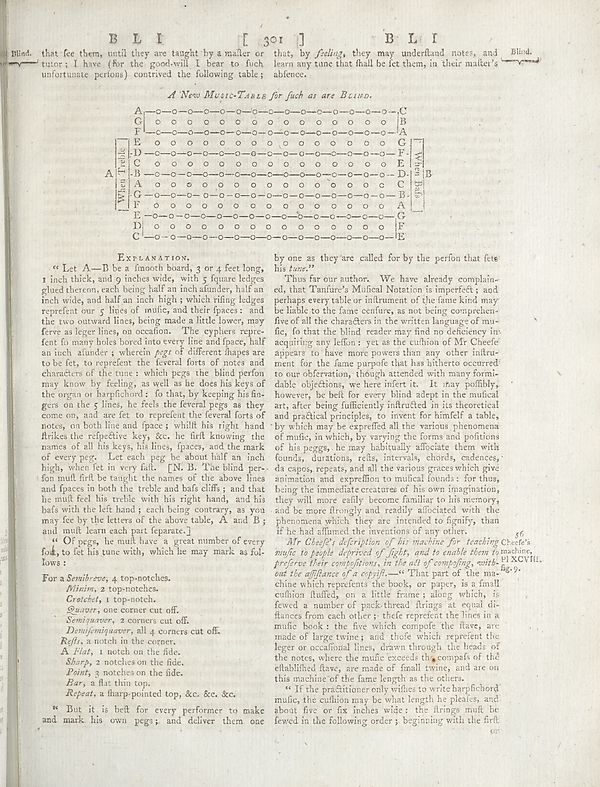
\includegraphics[width=0.85\textwidth]{../scans/page-2155-e6a255b57f58.jpg}
\caption*{Source scan: \texttt{page-2155-e6a255b57f58.jpg}}
\end{figure}

\end{document}
